\chapter{Background}
\label{sec:background}

\reversemarginpar

We review modeling and inference in BNs and in DNs.

\section{Bayesian Networks}
\label{sec:baysian_networks}

Let $U = \{ v_1, v_2, \ldots , v_n \}$ be a finite set of variables, each with a finite domain.
A singleton set $\{v\}$ may be written as $v$, $\{ v_1, v_2, \ldots, v_n \}$ as $v_1 v_2 \cdots v_n$, and $X \cup Y$ as $XY$.
For disjoint $X,Y \subseteq U$, a \emph{conditional probability table} (CPT) $P(X|Y)$ is a potential over $XY$ that sums to one for each value $y$ of $Y$.

A \emph{Bayesian network}\marginnote{\tiny BAYESIAN NETWORK} (BN) \cite{pear88} is a \emph{directed acyclic graph} (DAG) $\cal{B}$ on $U$ together with CPTs $P(v_1 | Pa(v_1))$, $P(v_2|Pa(v_2)),$$\ldots,$ $P(v_n|Pa(v_n))$, where the \emph{parents} $Pa(v_i)$ of $v_i$ are those $v_j$ such that $(v_j,v_i) \in \cal{B}$.
We call $\cal{B}$ a BN, if no confusion arises.
Figure \ref{fig:dag} shows a BN with CPTs $P(fo)$, $P(bp)$,$P(lo|fo)$, $P(do|bp,fo)$, and $P(hb|do)$ are shown.
The \emph{d-separation method}\marginnote{\tiny D-SEPARATION} \cite{pear88} can be used to read independencies from a DAG.

\begin{figure}[hbt]
    \begin{center}
        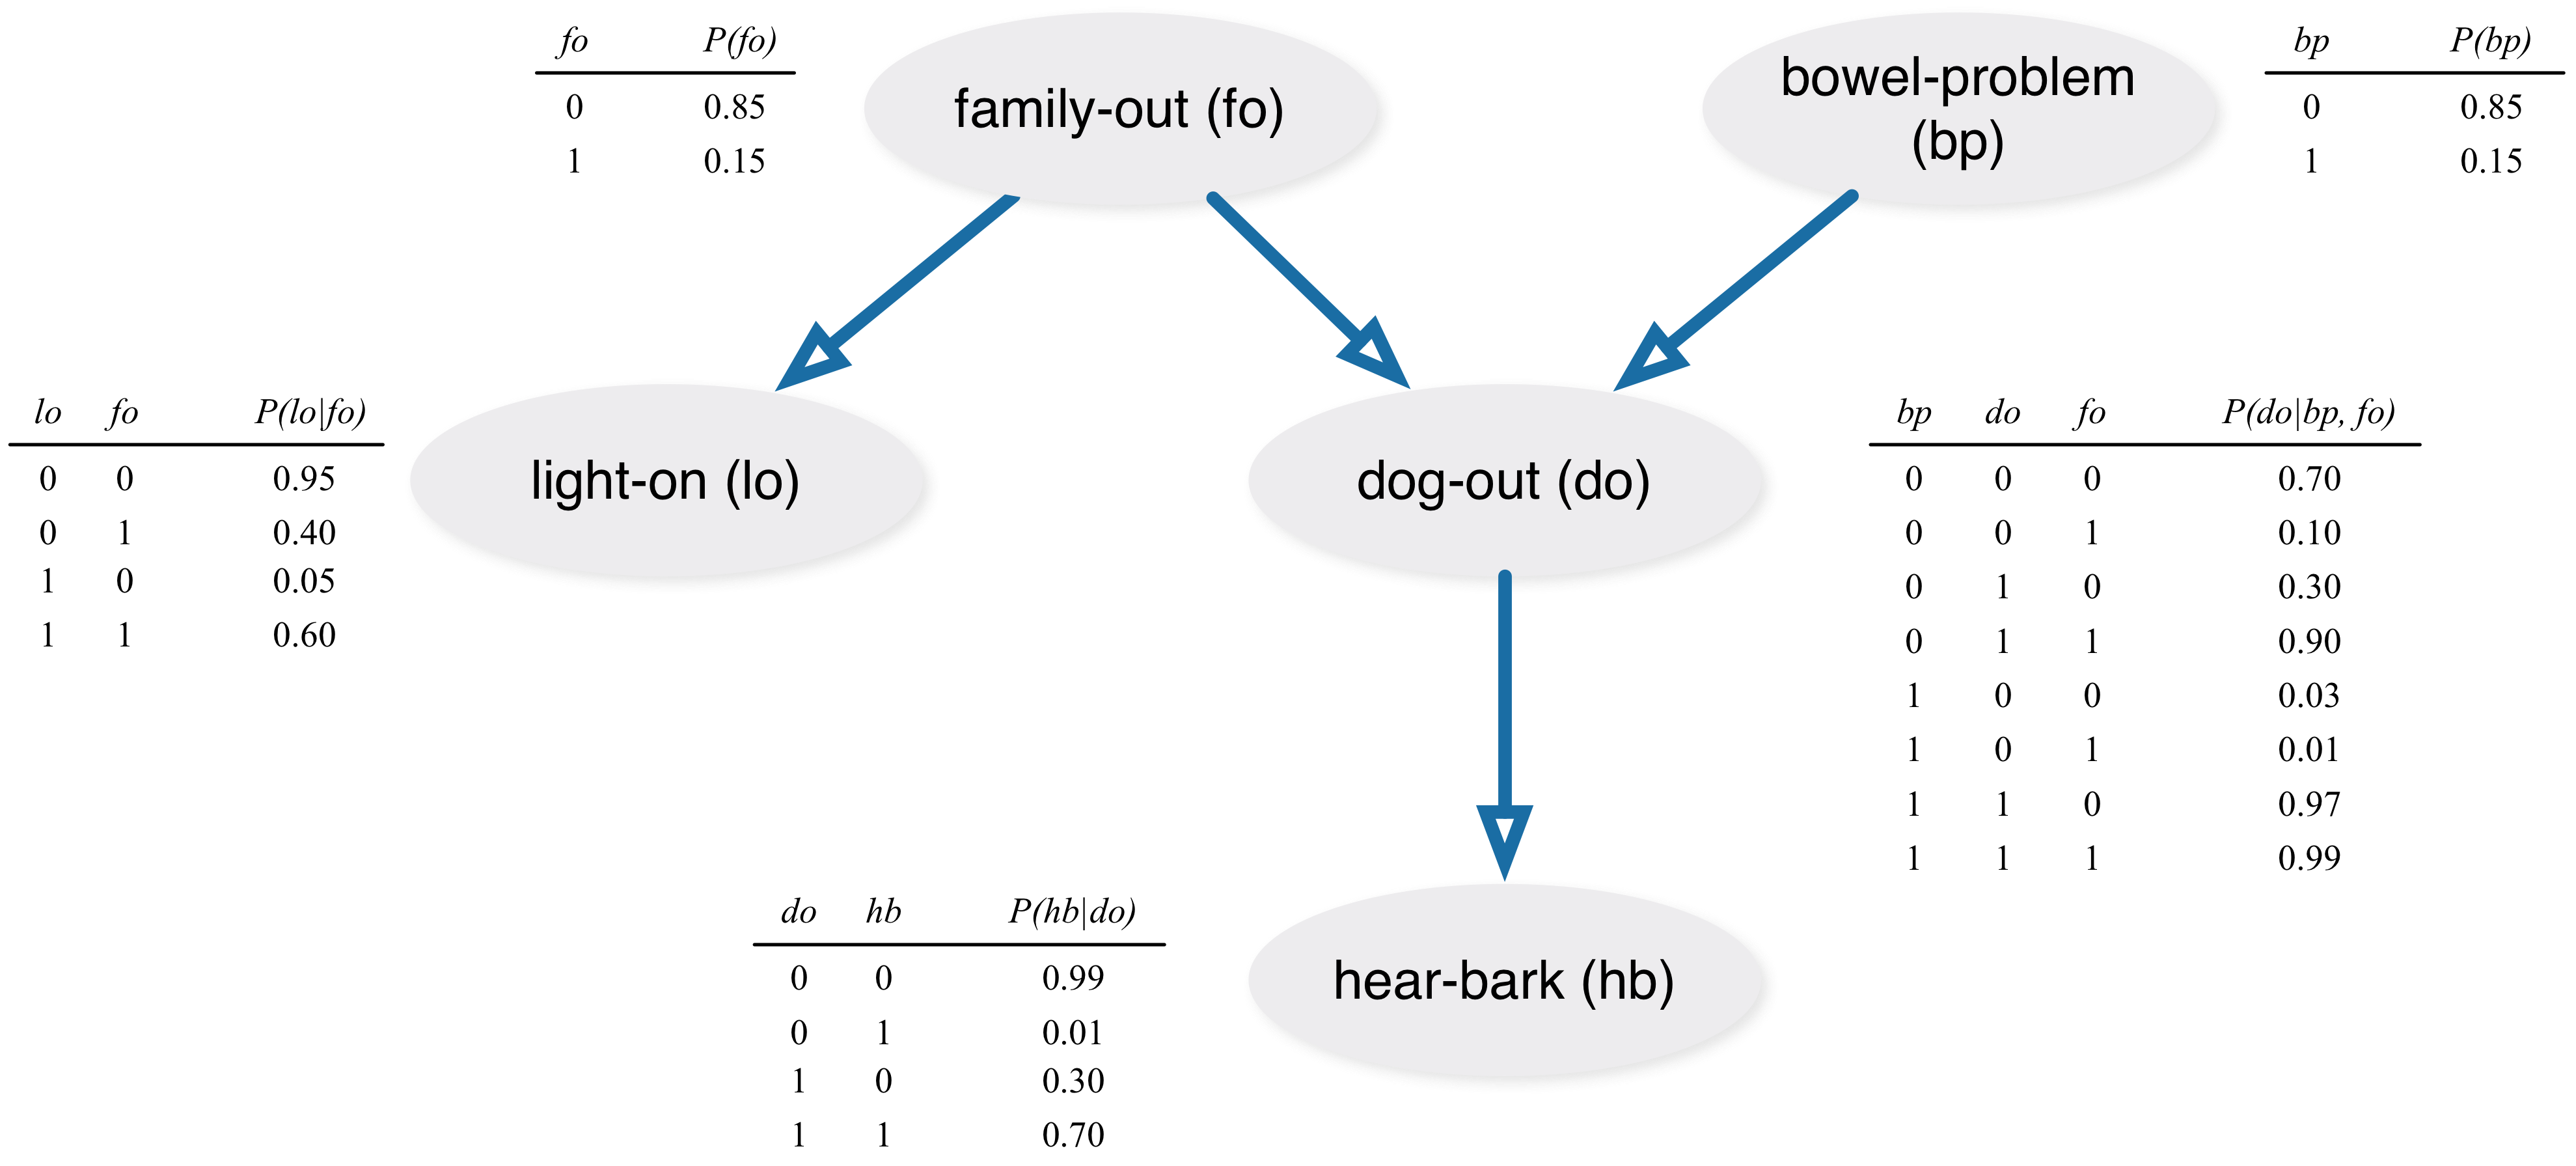
\includegraphics[width=\textwidth]{img/DAG_darwiche}
    \end{center}
    \caption{A DAG ${\cal B}$ and CPTs from \cite{darwiche09}.}
    \label{fig:dag}
\end{figure}

One method to perform inference on a DAG is called \emph{Variable elimination}\marginnote{\tiny VARIABLE ELIMINATION} (VE) \cite{zhan94}, which computes $P(X|Y=y)$ from a BN $\cal{B}$ as follows:
(i) all barren variables are removed recursively, where $v$ is \emph{barren} \cite{zhan94}, if $Ch(v) = \emptyset$ and $v \not\in XY$;
(ii) all independent by evidence variables are removed, giving ${\cal{B}}^s$, where $v$ is an \emph{independent by evidence} variable, if $I(v,Y,X)$ holds in $\cal{B}$ by m-separation;
(iii) build a uniform distribution $1(v)$ for any root of ${\cal{B}}^s$ that is not a root of $\cal{B}$;
(iv) set $Y$ to $Y=y$ in the CPTs of ${\cal{B}}^s$;
(v) determine an elimination ordering $\sigma$ from the moral graph ${\cal{B}}^{s}_{m}$;
(vi) following $\sigma$, eliminate variable $v$ by multiplying together all potentials involving $v$, and then summing $v$ out of the product;
and, (vii) multiply together all remaining potentials and normalize to obtain $P(X|Y=y)$.


To perform probabilistic inference, a BN is commonly transformed into a \emph{Markov network} \marginnote{\tiny MARKOV NETWORK}(MN) \cite{pear88}, also called a \emph{decomposable} MN. 
A MN consists of a triangulated (chordal) graph together with a potential defined over each maximal clique of triangulated graph. 
Given a DAG ${\cal D}$, the \emph{moralization} \cite{laur88} of ${\cal D}$ is the undirected graph constructed by adding an undirected edge between each pair of parents of a common child and then dropping directionality.
When necessary, edges are added to the moralized graph to obtain a triangulated graph. 
The maximal cliques are organized as join tree $\cal T$. 
Finally, the CPTs of the BN are assigned to nodes of $\cal T$. 


%\clearpage

\section{Darwinian Networks}
\label{sec:darwinian_networks}

\emph{Darwinian networks} (DNs)\marginnote{\tiny DARWINIAN NETWORKS} \cite{butzOliveiraSantosCai15} were proposed to simplify working with \emph{Bayesian networks} (BNs) \cite{pear88}.
Rather than modeling the variables in a problem domain, DNs represent the probability tables in the model.
The graphical manipulation of the tables then takes on a biological feel, where a CPT $P(X|Y)$ is viewed as the novel representation of a \emph{population} $p(C,D)$ using both \emph{combative} traits $C$ (coloured clear) and \emph{docile} traits $D$ (coloured dark).

\begin{figure}[hbt]
    \begin{center}
        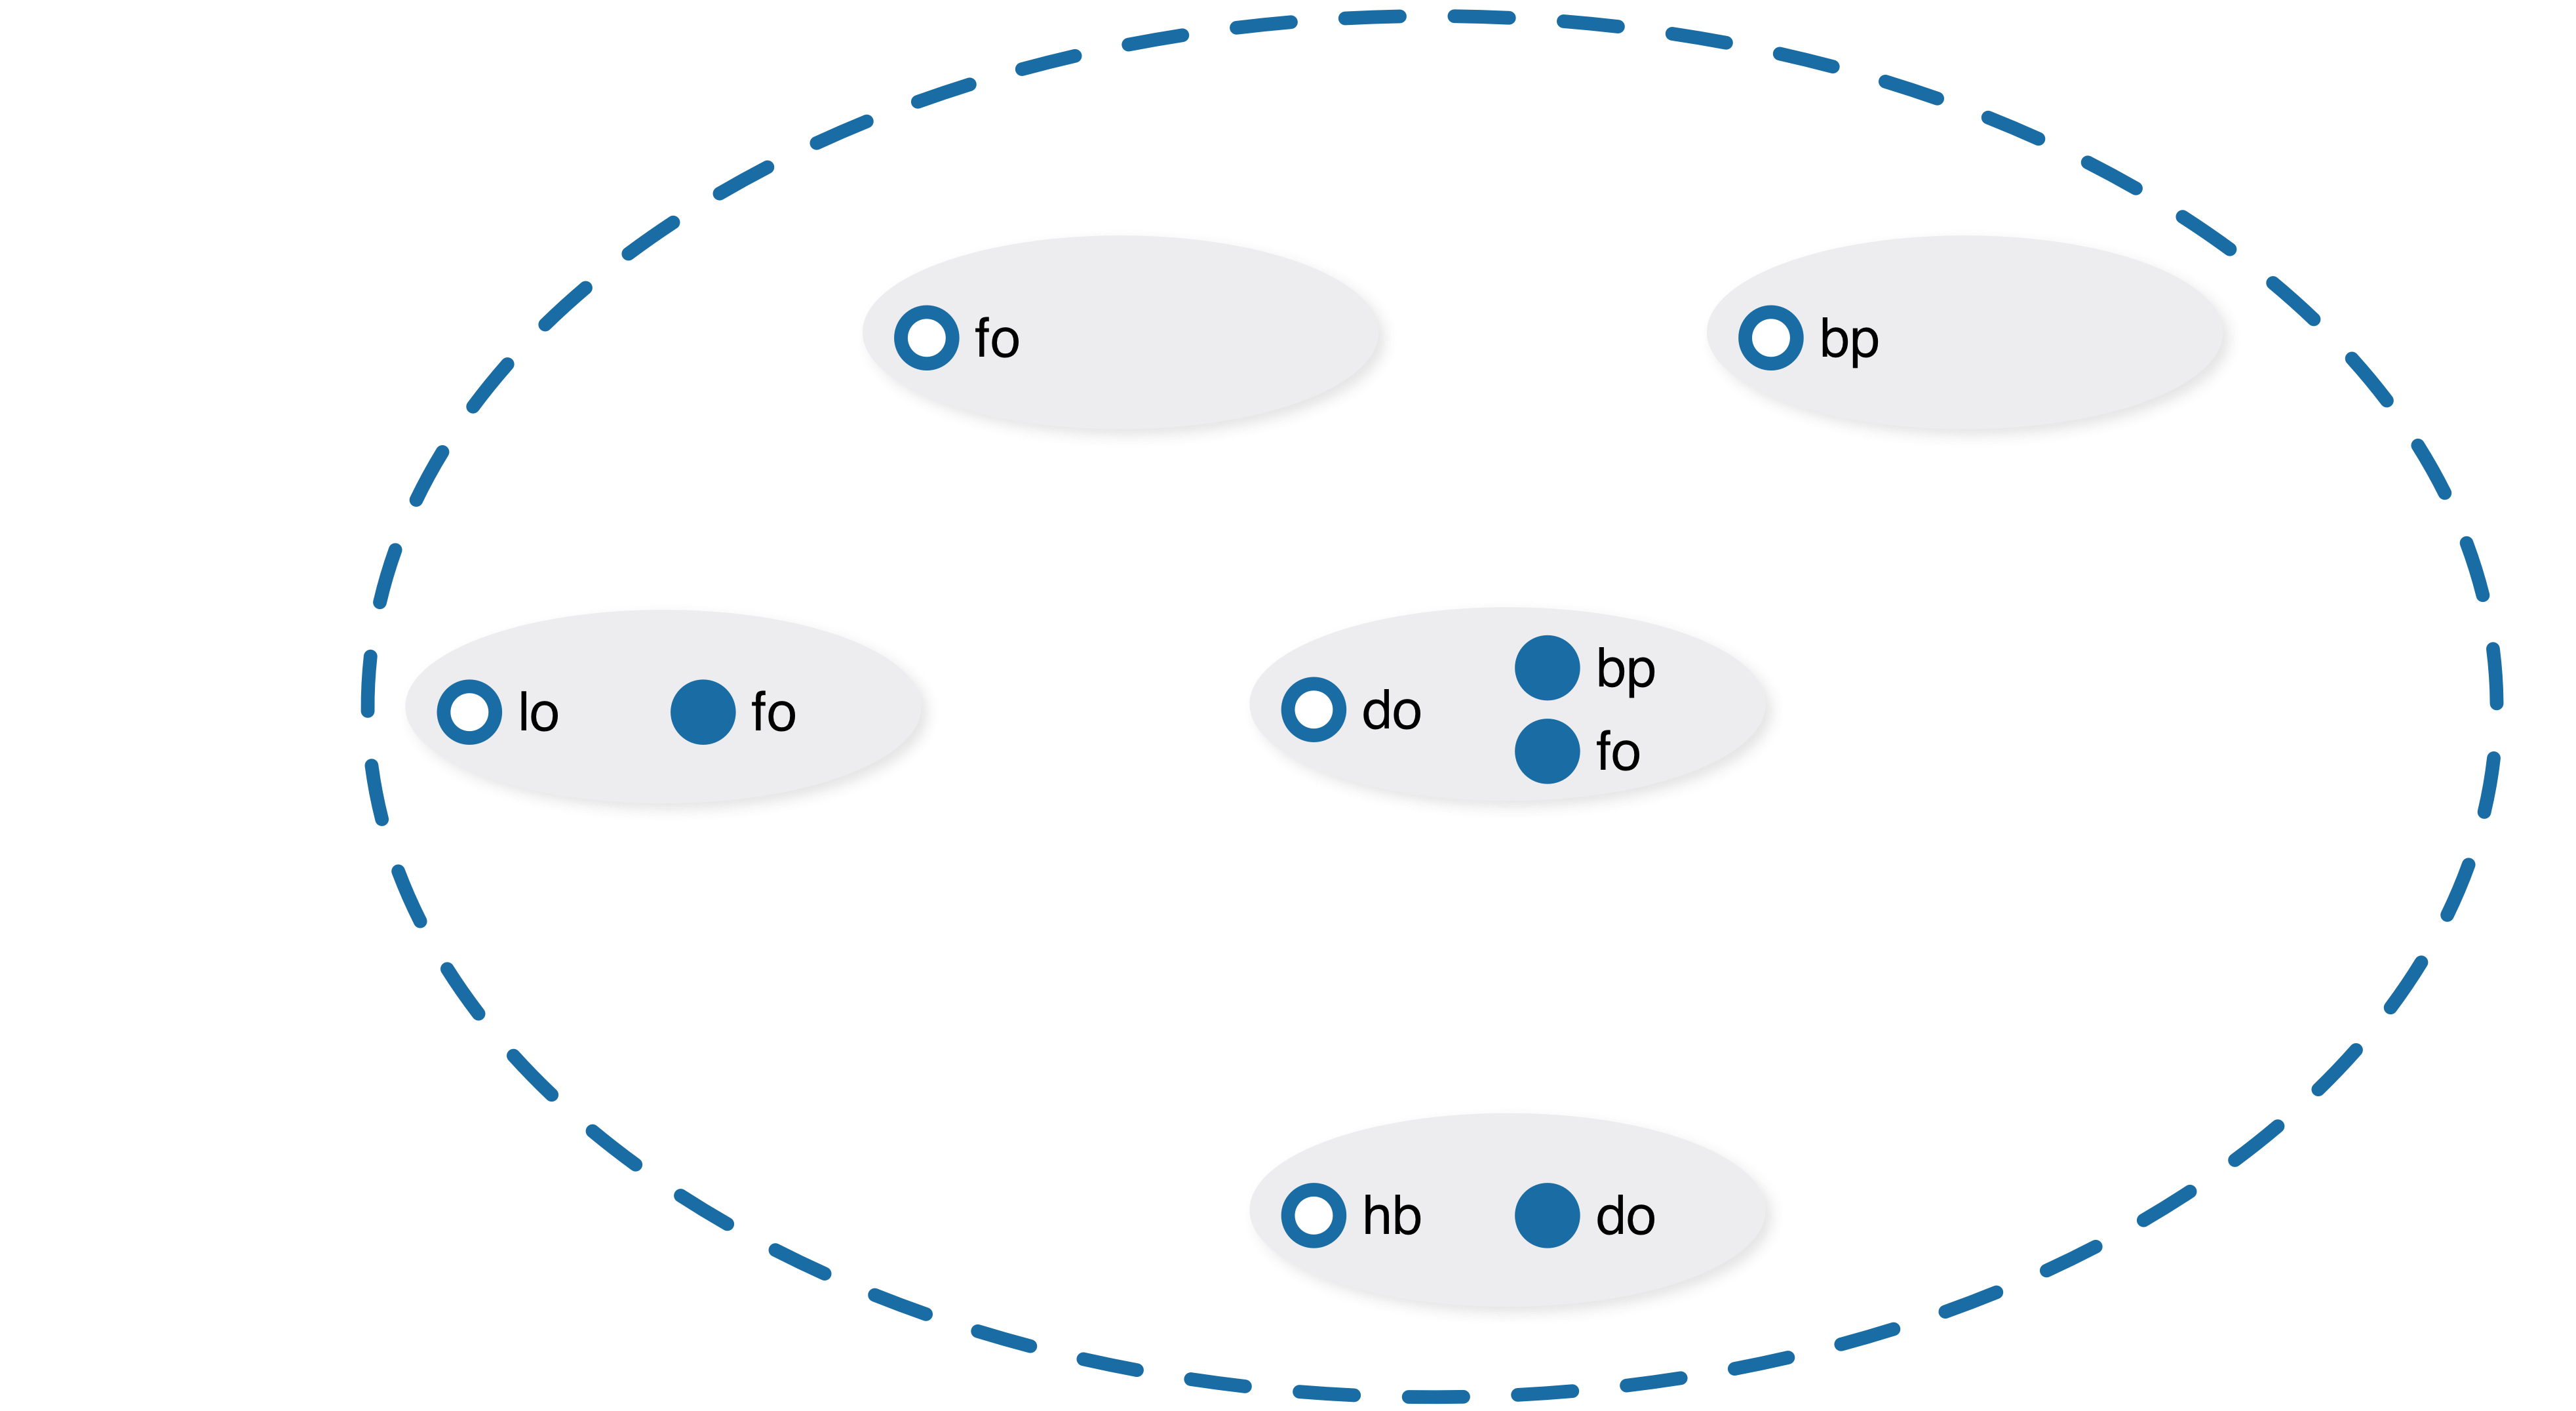
\includegraphics[width=\textwidth]{img/DN_darwiche}
    \end{center}
    \caption{A DN ${\cal D}$ representing DAG ${\cal B}$ of Figure \ref{fig:dag}.}
    \label{fig:dn}
\end{figure}

Adaptation and evolution are used to represent the testing of independencies and inference, respectively.
Thus, DNs can represent exact inference VE, as well the test of independencies d-separation.
Hence, DNs can unify modeling and reasoning tasks into a single platform.
The query $P(X|Y)$ posed to a BN ${\cal B}$ is represented by DN ${\cal D}^{\prime} = \{ p(X,Y) \}$ and the test of independence $I_{\cal{B}}(X,Y,Z)$ holds in a BN $\cal{B}$ if and only if tha adaptation $A({\cal{P}}_X, {\cal{P}}_Y, {\cal{P}}_Z)$ succeeds in the DN $\cal{D}$ for $\cal{B}$.



\subsection{Definitions}
\label{subsec:definitions}


%TRAIT

		A \emph{trait}\marginnote{\tiny TRAIT} $t$ can be combative or docile.
		A \emph{combative} trait $t_c$ is depicted by a clear (white) circle.
		A \emph{docile} trait $t_d$ is illustrated by a dark (black) circle.

%POPULATION

		A \emph{population}\marginnote{\tiny POPULATION}  $p(C,D)$ contains a non-empty set $CD$ of traits, where $C$ and $D$ are disjoint, $C$ is exclusively combative, and $D$ is exclusively docile.
		A population is depicted by a closed curve around its traits.

%DN

		A \emph{Darwinian network} (DN)\marginnote{\tiny DN} , denoted $\cal{D}$, is a finite, multiset of populations.
		A DN $\cal{D}$ is depicted by a dashed closed curve around its populations.
		All combative traits in a given DN $\cal{D}$ are defined as $T_c(\cal{D})$ $=$ $\{t_{c} ~ | ~ t_{c} \in C,$ for at least one $p(C,D) \in \cal{D}\}$.
		All docile traits in $\cal{D}$, denoted $T_d(\cal{D})$, are defined similarly


\subsection{Operations}
\label{subsec:operations}



%		DOCILIZATION
		
		\emph{Docilization}\marginnote{\tiny DOCILIZATION} of a DN $\cal{D}$ adds $p(\emptyset,D)$ to $\cal D$, for every population $p(C,D)$ in ${\cal D}$ with $|D| > 1$.
		

%		DELETION
		
		To \emph{delete}\marginnote{\tiny DELETION} a population $p(C,D)$ from a DN $\cal{D}$ is to remove all occurrences of it from $\cal{D}$.
		

%		MERGE
		
		Two populations \emph{merge}\marginnote{\tiny MERGE} together as follows: for each trait $t$ appearing in either population, if $t$ is combative in exactly one of the two populations, then $t$ is combative in the merged population; otherwise, $t$ is docile.
		

%		NATURAL SELECTION
		
		In adaptation, \emph{natural selection}\marginnote{\tiny NATURAL SELECTION} removes recursively all barren populations from a DN $\cal{D}$ with respect to another DN ${\cal{D}}^{'}$.
		

%		REPLICATION
		
		\emph{Replication}\marginnote{\tiny REPLICATION} of a population $p(C,D)$ gives $p(C,D)$, as well as any set of populations $p(C^{'}, D)$, where $C^{'} \subset C$.
		

\subsection{Adaptation}
\label{subsec:adaptation}


In DNs, how populations ``adapt'' to the deletion of other populations corresponds precisely with testing independencies in BNs.

Let ${\cal{P}}_X$, ${\cal{P}}_Y$, and ${\cal{P}}_Z$ be pairwise disjoint subsets of populations in a DN $\cal D$ and let DN ${\cal{D}}^{'} = {p(C)}$, where $C = T_c({\cal{P}}_X {\cal{P}}_Y {\cal{P}}_Z)$. 
The test \emph{adaptation}\marginnote{\tiny ADAPTATION} of ${\cal{P}}_X$ and ${\cal{P}}_Z$ given ${\cal{P}}_Y$, denoted $A({\cal{P}}_X,{\cal{P}}_Y,{\cal{P}}_Z)$, in $\cal D$ with four simple steps:
(i) let natural selection act on $\cal{D}$ with respect to ${\cal{D}}^{'}$, giving ${\cal{D}}^{s}$;
(ii) construct the docilization of ${\cal{D}}^{s}$, giving ${\cal{D}}^s_m$;
(iii) delete $p(C,D)$ from ${\cal{D}}^s_m$, for each $p(C,D)$ in ${\cal{P}}_Y$; and,
(iv) after recursively merging populations sharing a common trait, if there exists a population containing both a combative trait in $T_c({\cal{P}}_X)$ and a combative trait in $T_c({\cal{P}}_Z)$, then $A({\cal{P}}_X,{\cal{P}}_Y,{\cal{P}}_Z)$ fails; otherwise, $A({\cal{P}}_X,{\cal{P}}_Y,{\cal{P}}_Z)$ succeeds.


\subsection{Evolution}
\label{subsec:evolution}


The \emph{evolution}\marginnote{\tiny EVOLUTION} of a DN $\cal{D}$ into a DN ${\cal{D}}^{'}$ occurs by natural selection removing recursively all barren, independent, and spent populations, merging existing populations, and replicating to form new populations.


